\chapter{Experiments}
The main purpose of this chapter of this paper is to compare animations
generated procedurally with the use of Ik with baked animations. The comparison
is broken up into two categories - visual and performance. 

\section{Baked animations}
 In order to conduct the experiments comprised of visual and performance
 comparisons, a second set of animations were created each of the examples which
 are shown in the demo application. Below is an explanation of the process of
 creating this second set of animations.

\subsubsection{Spider}
The baked animation version of the spider was animated in Blender. The set
consists of idle and walking animations which, in Blender, are placed on
a single timeline, one after the other (Figure \ref{fig:timeline}). Once the model is imported
into Unity, the animations can be broken up into their separate cases, as shown
earlier in the "tools" chapter of this paper (Figure \ref{fig:anim_chunk}). 

\begin{figure}[h!]
    \centering
    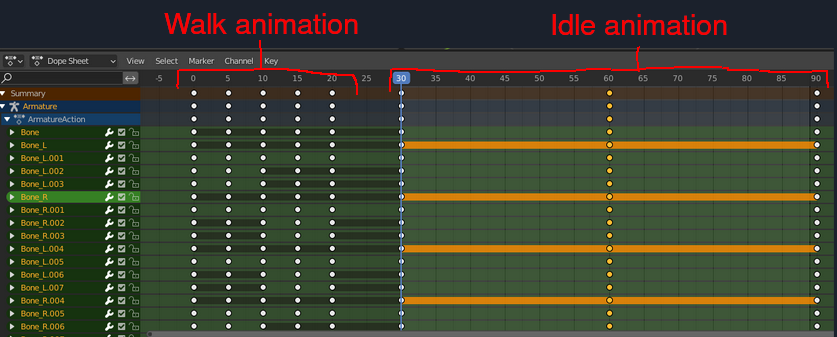
\includegraphics[width=0.7\textwidth]{grafika/blender_timeline.png}
    \caption{Two animations on a single timeline}
    \label{fig:timeline}
\end{figure}

Once the animations have been imported, a new animation controller is created
for the new spider. The animations are added, this time with the use of a blend
tree (Figure \ref{fig:s_blendtree}) to, as the name suggests, blend between the
animation smoothly CITE. A third animation state is added to the blend tree
which is the equivalent of the walking animation, but the animation speed is set
to a negative value. This plays the animation in reverse and is used when the
spider is walking backwards. 

\begin{figure}[h!]
    \centering
    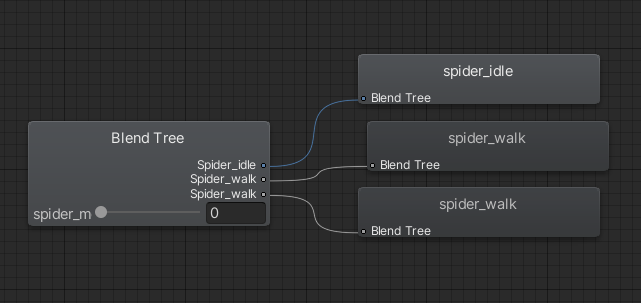
\includegraphics[width=0.7\textwidth]{grafika/spider_blend.png}
    \caption{Blend tree containing animations for the spider}
    \label{fig:s_blendtree}
\end{figure}

A variable named \textit{spider\_movement} is created in order to control the
animations that are to be played in a given situation, and the manner in which
the transitions should be blended. The thresholds for each animation can be
defined in the blend tree's configuration in the animator (Figure ref).

\begin{figure}[h!]
    \centering
    \captionsetup{justification=centering}
    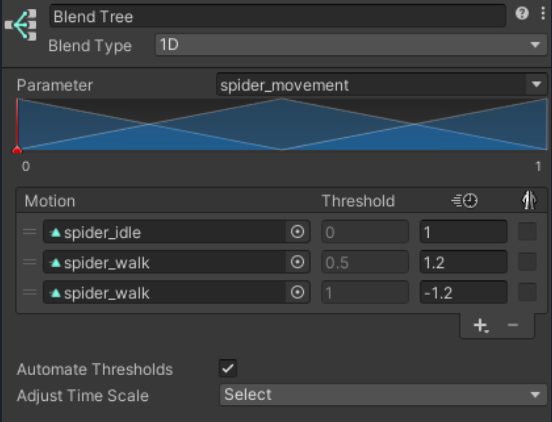
\includegraphics[width=0.7\textwidth]{grafika/spider_blendconf.png}
    \caption{Configuration of the spider's blend tree which is dependent on
    the \textit{spider\_movement} variable}
    \label{fig:s_blendconf}
\end{figure}

In the spiders movement script, this variable can then be set in reaction to
certain inputs so that the proper animation is activated each given situation.
To achieve the transition blending, the \textit{spider\_movement} variable
should not be set outright to the value which corresponds to the next animation
state. Instead, the \textit{\_animator.SetFloat} method is used, where the
\textit{\_animator} is a reference to the spider's Animator component. This
method allows the value of spider\_movement to be interpolated from the value of
the current animation state to another desired value.
\newline
\begin{lstlisting}[basicstyle=\footnotesize, numbers=none,frame=single,
caption={Transitioning to the spider's idle animation using the
\textit{SetFloat} method},captionpos=b, label=stretch, language={[Sharp]c}]
    if (verticalAxis == 0f && horizontalAxis == 0f)
        _animator.SetFloat("spider_movement", 0f, 0.05f, Time.deltaTime);
\end{lstlisting}

This version of the spider has its movement based on the spider from the game
Minecraft, which means that its rotation on the x and z axes is locked. The
spider can rotate about the y-axis when turning to face a different direction,
but it will not adjust to variations in the surface which it walks upon.
Additionally, when the spider encounters a vertical wall, it begins moving
vertically instead of horizontally until it scales the entire obstacle.

\subsubsection{Human}
The baked version of the human character, which performs an animation sequence
consisting of pressing buttons, is animated in Blender. The animation plays one
full sequence of pressing a single button. Chunks of the same animation are used
in the IK version of this animation sequence, described in the previous chapter,
but the baked animation uses the full animation while the IK version uses only
the beginning and the end. However, the animation is still broken up into three
parts when imported into Unity: the raising of the hand, the button pressing
motion, and the lowering of the hand (Figure \ref{fig:bp_clips}). This is done
because when the character is pressing multiple buttons in a row, the hand
should not be lowered to its starting position after every press.

\begin{figure}[h!]
    \centering
    \captionsetup{justification=centering}
    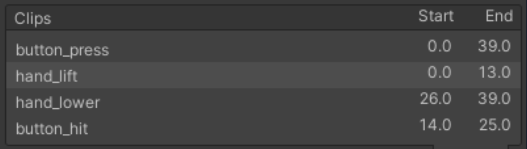
\includegraphics[width=0.7\textwidth]{grafika/bp_clips.png}
    \caption{The full button press animation is broken up into 3 separate clips}
    \label{fig:bp_clips}
\end{figure}

Another animation controller is created for this version of the human. Unlike
the spider example, the animation states do not have to be blended as they are
all clips which combine to create the full button press animation, and the
transitions are seamless as they are. Because of this, the animation states for
the three animation clips are not part of a blend tree, and instead are just
"floating" states with no defined transitions. The logic for which animation
should be played at what time is defined in the main script attached to the
character. 

The script is a simplified version of the one which controls the IK version of
this character's animation. It has no need for the public parameters present in
it's IK version because there is no IK rig, IK target, or button transforms
which it needs to control. Due to this, there is no list containing the sequence
of buttons to be pressed. It is instead replaced by an integer value which
dictates the number of button presses to execute in one animation sequence in
order to convey the idea that the character is pressing multiple buttons in
a sequence. 

As with the IK version of this script, the logic is based on a set of coroutines
which control the flow of the animation sequence. However, only the
\textit{HandAnimation} coroutine is used as a building block for the sequence
because the whole action is now constructed using baked animations. When the
script receives an input and the animation is not already playing, the sequence
begins by setting the \textit{idle} variable to true to prevent the sequence
from being repeated while it is still in progress. All required animation clips
are then set off one after the other, starting with the animation to lift the
hand. This is then followed by the animation clip which is responsible for
hitting the button, and it is repeated in a loop for a number of times defined
by the button press count parameter. Finally, the animation clip for lowering
the hand is executed, and the \textit{idle} boolean is set to false before
terminating the sequence.

\section{Visual Comparison}
The goal of using inverse kinematics to procedurally animate a model in video
games is to achieve a more natural interaction between a character and the
environment. The realism of the interaction is conveyed through how it looks,
and how the animation is a more realistic representation of how such an action
might look in real life. Therefore, the visual integrity of the IK animation as
it adapts to a plethora of scenarios is what sets it apart from a classic
approach through baked animations. 

\subsubsection{Spider}
The walking animation, or any basic movement animation, is the core of what
most characters will be doing a majority of the time. That being the case,
a natural movement animation will contribute the most to the overall look and
feel of the character. This difference can be clearly noticed by comparing the
two version of the spider implemented in the demo application created for the
purpose of this paper. 

Starting with the idle position, both models look quite natural standing on
a flat surface, as seen in Figures ref and ref (one figure with two images).

However, this changes when as soon as the surface is uneven. The IK acting on
the legs of the spider in Figure ref is able to use its ray casts to match the
surface exactly, while the baked version of the spider doesn't have this
mechanism, and its legs can be seen floating in the air (Figure ref). The same
effect is observed when the spider is moving. The baked version's legs float
when it is moving over uneven or slanted surfaces, which gives it an effect as
if the spider was swimming through the air. 

Another difference between the two spiders is how they climb walls. Whereas the
IK version is able to treat it the same as any other surface, the baked version
keeps does not adjust its rotation, and instead climbs the wall head on (Figure
ref). This kind of rotation could have been implemented, however, the transition
between floor and wall would be very unnatural either way and so an
implementation inspired by the spiders in the popular game Minecraft was used
instead.

One important aspect to note when comparing the realism of both animations is
how the legs move relative to the surface on which they stand. In the case of
the procedural animation, the IK targets controlling the spider's legs remain
fixed in one place until a leg movement is initiated. As a result, no matter the
speed at which the spider is moving, the give the impression that they are
placed on the floor and push away realistically. On the contrary, the baked
animation is played at a certain speed, and it is very hard to match the
animation speed to the movement speed so that the legs seem to stay in a fixed
position on the ground while the spider is moving. This breaks the illusion of
the legs pushing the spider forwards, as they instead glide on the surface out
of sync.

\subsubsection{Human}
In a game where pressing buttons is not a core mechanic, the accuracy of such an
animation sequence may not be important, and a generic animation can be used to
convey the idea. However, in the event that the sequence of the buttons is
important, such as a player needing to provide a specific input to hack a code
to open a door, the realism of the game can be elevated through the use of
inverse kinematics. The adaptability of a character's action can be seen in this
comparison between the baked and IK versions of the button press animation.

When the character is only required to press a single button, while also having
a proper position and orientation relative to the button, the baked animation
looks quite natural, and looks no different than the IK version (Figure ref)

The difference start to be noticeable when the character is offset or rotated
from the default position. While the IK target leads the hand correctly to the
button (Figure ref a), the baked animation has no knowledge of the characters
surroundings, and misses its mark (Figure ref b). Due to this, for realism to be
preserved when using a baked animation, either the character must be reoriented
as part of the action, or a cutscene should be played for the duration of the
action. 

The next benefit of the procedural animation is its ability to adapt to a panel
with multiple buttons. A seen in Figure ref, the IK target leads the hand to the
appropriate position for each separate button. This allows for a specific
sequence of buttons - taking the door hacking example from before this would be
a player's input - to be pressed in a way which visually conveys the exact
action which was commanded, in a responsive manner.

Comparing this to the baked animation sequence, the character is only able to
aim its hand at one specific point, consequently missing all the buttons (Figure
ref). In the case of a sequence of buttons being pressed, the character repeats
the press in a single spot which doesn't realistically convey the pressing of
a sequence of buttons. This can be slightly improved by constructing the
animation to aim at different buttons on the panel in a generic order. The
downside of this patch is that it falls apart if there is a change in the amount
of buttons, or their positions and configuration. 



\section{Performance Comparison}

\subsubsection{Spider}
\subsubsection{Human}
